\chapter{背景 Background}
\label{background}

% not so sure %
% In this section we put game design and NDN side by side and summarize concepts, from both realm, that are most closely related to consistency, scalability and security.

%-----------------------------------%
\section{Game Design Background}
\label{gamedesignbg}

% (scalability -- architecture)  (consistency -- synchronization algorithm) %
The scalability of a system is closely related to its architecture. In an unscalable architecture, when the client number increases resource bottlenecks would appear, reducing system overall performance. Depending on which architecture is used, a system may need a synchronization mechanism to maintain consistency. Security and cheating avoidance strategies are also architecture-dependent.

% . . . . . . . . . . . . . . . . . . . . . . . %
\subsection{Game Architectures}
\label{game_archi}

% C/S and P2P %
Game architecture are usually classified as Client\slash Server (\cs) or peer-to-peer (P2P). 

In {\cs} architectures (figure~\ref{cs}) all clients are connected to a central server which receives client events, authenticate, compute and publish updates of global game state. The only two responsibilities of clients are sending user input to the server and rendering the new game state received from it. This centralized model intrinsically guarantees consistency, as there is only one source of global game state. However, the server is also the resource bottleneck, rendering the system unscalable. This architecture is not robust as the server is a single point of failure. Finally the server introduces additional latency.

In contrast, in P2P architectures (figure~\ref{p2p}) there is no central authority. Clients, or peers are interconnected with each other and each peer maintains its own copy of the game state. Player authentication and game state computation are decentralized and peers send messages asynchronously to inform updates. Because P2P architectures resource-growing~\cite{Scheating}, they are scalable. Because peers send messages directly to each other, network latency is minimized. However, P2P architectures require synchronization mechanisms to guarantee the consistency of the replicated game state among peers. Cheating is also easier in P2P than it is in {\cs}.

\begin{figure} 
\centering  
\subfigure[\cs]  
{  
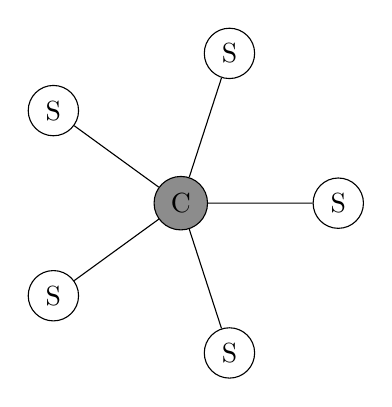
\begin{tikzpicture} [scale=1, transform shape]
\tikzstyle{every node}=[draw,shape=circle];
\node [fill = gray!90] (v0) at (0:0) {C};
\node (v1) at ( 0:2) {S};
\node (v2) at ( 72:2) {S};
\node (v3) at (2*72:2) {S};
\node (v4) at (3*72:2) {S};
\node (v5) at (4*72:2) {S};
\draw (v0) -- (v1) % star
(v0) -- (v2)
(v0) -- (v3)
(v0) -- (v4)
(v0) -- (v5);
\end{tikzpicture}
\label{cs}
}  
\subfigure[P2P]  
{  
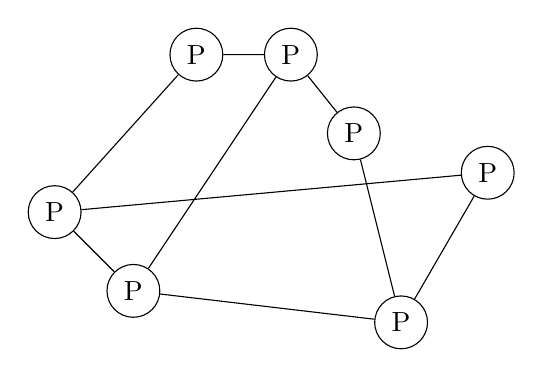
\begin{tikzpicture} [scale=1, transform shape]
\tikzstyle{every node}=[draw,shape=circle];
\node (v0) at (0, 2) {P};
\node (v1) at (1, 1) {P};
\node (v2) at (1.8, 4) {P};
\node (v3) at (3, 4) {P};
\node (v4) at (4.4, 0.6) {P};
\node (v5) at (3.8, 3) {P};
\node (v6) at (5.5, 2.5) {P};
\draw (v0) -- (v1)
(v0) -- (v2)
(v0) -- (v6)
(v4) -- (v5)
(v1) -- (v4)
(v2) -- (v3)
(v3) -- (v5)
(v4) -- (v6)
(v3) -- (v1);
\end{tikzpicture}
\label{p2p}
}
\caption{\cs~and P2P architectures}
\end{figure}

Hybrids of {\cs} and P2P exist: Mirrored Game Servers, Distributed Scene Graphs and many more. These architectures are described in~\cite{Ldsg, Scheating, Fgame, Csync}.


% . . . . . . . . . . . . . . . . . . . . . . . %
\subsection{Synchronization Mechanisms}
\label{syncalgr}

% conservative and optimistic %
The simplest way to maintain consistency among peers is to use totally ordered service, which is often not available. Therefore conservative and optimistic synchronization algorithms have been proposed to prevent or detect (and then correct) misorderings~\cite{Fgame}. 

Conservative synchronization algorithms would allow each peer to process received events only if it is safe to process them. Newly arrived events are usually delayed for an amount of time and the synchronization algorithm can determine the correct execution order. Famous examples are \emph{Chandy-Misra-Bryant algorithm}~\cite{Chandy, Bryant}, \emph{Lockstep synchronization}~\cite{Flockstep} and \emph{fixed time-bucket synchronization}. % Conservative algorithms do not exploit concurrency well and the delay they introduce will reduce interactivity.

Optimistic synchronization algorithms assume received events are in correct order and process them without delay. Then, if late events arrived a \emph{rollback} will be performed and all those optimistically executed events should be canceled and reprocessed. In order to rollback, large memory will used to take multiple snapshots of game state. Also, a mechanism to determine the early bound of rollback (for example the \emph{Global Virtual Time}) will be mandatory. The most famous optimistic synchronization algorithms are: \emph{Time Warp}, \emph{trailing state synchronization}~\cite{Csync}~and \emph{optimistic time-bucket synchronization}~\cite{Doptbkt}.

%-----------------------------------%
\section{NDN Background}
\label{ndnbg}

% Basic Exchange %
NDN \emph{names} can be human-readable (for example \url{/Egal/Car/Scene0}). Their binary encodings can be used for routing using longest prefix match.

NDN is designed for content distribution. Two packet types exists in NDN: \emph{Interest} and \emph{Data} (see figure~\ref{packet_types}). A data receiver first initiates an Interest packet that bears the \emph{name} of the \emph{content} it wants. The packet is then routed by name until it reaches a host that has the corresponding content. The matching content object is sent back as a Data packet, satisfying all Interest for it on its way and leaving a trail of `bread crumbs'~\cite{Jndn}~in the routers' memory. Later Interests for the same content may be directly satisfied by the routers. It is guaranteed that in NDN every piece of data would flow through a link for at most once. This would reduce a huge amount of network traffic around content distribution centers.

\begin{figure} 
\begin{center}
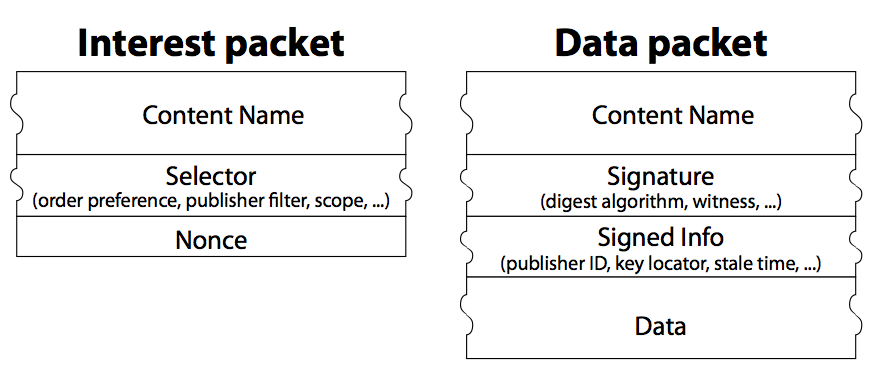
\includegraphics[width=0.7\textwidth] {images/packet_types}
\caption{packet types in NDN}
\label{packet_types}
\end{center}
\end{figure}

Note that NDN is receiver driven. Flow balance is also controlled by the receiver~\cite{Zact}. Also note that multicasting is intrinsically built in.

% . . . . . . . . . . . . . . . . . . . . . . . %
\subsection{CCNx Sync Protocol}
\label{ccnsync}

The CCNx Sync protocol allows applications to define collections of named data in \emph{repositories} that are to be automatically kept in sync with identically defined collections in neighboring repositories~\cite{CCNxSync}. A collection in the repository is also called a \emph{slice}. A local \emph{Sync Agent} builds and manages a \emph{Sync Tree} for a slice, using names that represent the content of the slice. Hashes of Sync Trees are sent among neighboring Sync Agents to detect any discrepancy. Once detected, normal Interest and Data packets will be sent for inconsistent data.

CCNx Sync protocol should not be confused with the game synchronization protocols mentioned in~\ref{syncalgr}. CCNx Sync maintains data integrity: it keeps local repository slices coherent remote ones. Game synchronization algorithms provide a higher level service: they ensure that sync actions will be taken \emph{in order}.

